To begin identifying an appropriate development methodology, it is necessary to understand the project requirements. The project requirements are determined over a number of meetings with the primary stakeholders. These meetings discuss the minimum requirements and the features that are going to be implemented on the project. 

At this point the development methodology can be determined. Since we are looking for iterative and incremental development, Agile Software Development Methodology will be followed. This also enables time-boxed iterative approach. Agile methods are focused on different aspects of the software development life cycle. Two of the most well known agile methodologies are Scrum and XP.

Scrum is a project management agile framework. It’s use focuses more on the management of software development projects. The product is completed in a series of one to four week iterations, or sprints. Before each sprint, a planning meeting is held to define which features will be implemented during that sprint. There are also daily 15 minute meetings where each member informs the group about what he did, what he will do and if he found any difficulties. 

Similarly, XP (Extreme Programming) is an agile methodology which focuses on the values of simplicity, communication, feedback, and courage. XP is designed for small, co-located teams aiming to get quality and productivity as high as possible. It does this through the use of rich, short, informal communication paths with emphasis on skill, discipline, and understanding at the personal level, minimizing all intermediate work products. 

As this is a college project and tight time constraints apply, it is quite
difficult to follow a particular methodology. Scrum focuses on the management
side of the project whereas XP focuses more on the actual programming
practices. It is more preferable if various elements from both methodologies
can be used since they address different areas and complement each other.

It was decided to focus on managing the software project using the scrum
approach and adopt it's characteristics that suit the project. The team is
composed of six students. Weekly meetings are planned to organise the division
of work and for the team to get up to speed with all the tasks in progress and
completed. An agenda for each meeting is stored in an online document, that
each team member may add to. 

To make the production more effective and faster, an online collaboration tool
"Trello" is used. This tool gives access to a visual board and displays all the
required short-term and long-term tasks, which are represented as cards with
various labels and priorities. This board is very similar in concept to the
scrum board as shown in fig 2.

\begin{figure}[here]
\begin{minipage}{\textwidth}
\begin{center}
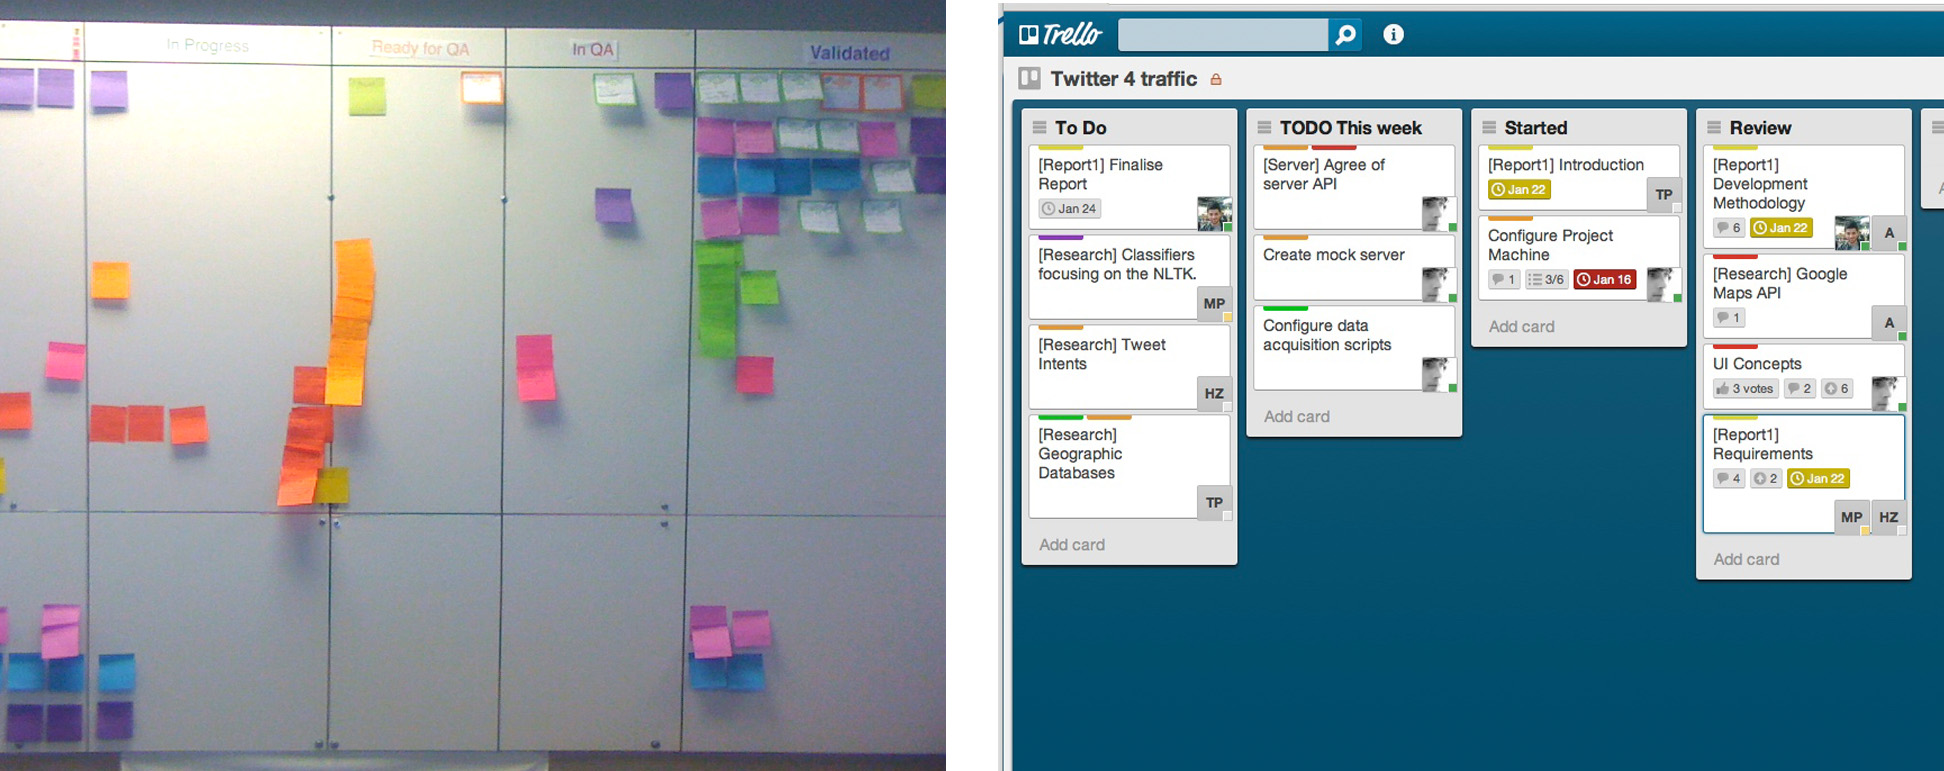
\includegraphics[width=0.8\textwidth]{images/scrumboard.jpg}
\end{center}
\vspace{-20pt}
\caption[Caption for LOF]{Scrum Board and Trello\footnotemark}
\end{minipage} 
\end{figure}


Adopting several techniques from the XP also seemed advantageous, helping to
improve the process. The first practise we decided to use is pair programming,
having two programmers work alongside on the same code. At any time, those two
programmers sitting together may change any line of code in the system. Any
time the two find a section of code that appears hard to understand or overly
complex, they are to revise it, constantly simplifying and improving it. This
technique improves the code quality and the team focus. Furthermore, several
tests will be added in our code-base, keeping a test-driven development.
However because of the nature of the project being partly research based and
the results being quite subjective, it is difficult to test effectively. Hence,
the development of the mobile application will be test-driven whereas for the
server development we won't be able to follow test-driven so strictly.\cite{Cockburn}

For the division of work amongst the project, more flexibility will be achieved by maximising the use of the members previous experience, but also keeping everyone interested. A balanced division has been decided where two members of the team will focus on the mobile application, two on the server side and the rest will move between those two tasks as necessary. However these movements have to be kept to the minimum because we are well aware of the Brook's Law which emphasizes that adding manpower to a late software project makes it later.\cite{Brooks}

To facility parallel development, the server API will be mocked-up and will produce a fixed data set in the desired format that the android applications can handle. That way, those developing the mobile application can work independently from those working on the server. One person on the team is designated as the team "coach". This person reviews with the team members their use of the key practices: use of pair programming and testing,keeping design simple, communicating, and so on.

As regards the actual design of the project there are multiple aspects. The first one is the mobile application that will act as the front-end of the system. For the user interface, some Lo-Fi layouts will be drawn in paper in order to have a general idea of how the interface is going to look like. The relative data will be retrieved in a structured form that will be the same for the server and the mobile application. The second aspect is the server implementation. A project machine will be used for the server, where traffic feeds from TFL and Twitter will be retrieved in XML format and stored in a database.

\footnotetext{Left: Drew Stephens \url{flickr.com/photos/dinomite/3695570625}, Right: \copyright \url{Trello.com}}
